\section{What is dynein?}
\textit{Introduce dynein as motor protein . Maybe just a quick single paragraph or two of background knowledge on motor proteins and compare it to kinesin and myosin. Basic functions}
\begin{figure}[H]
	\centering
	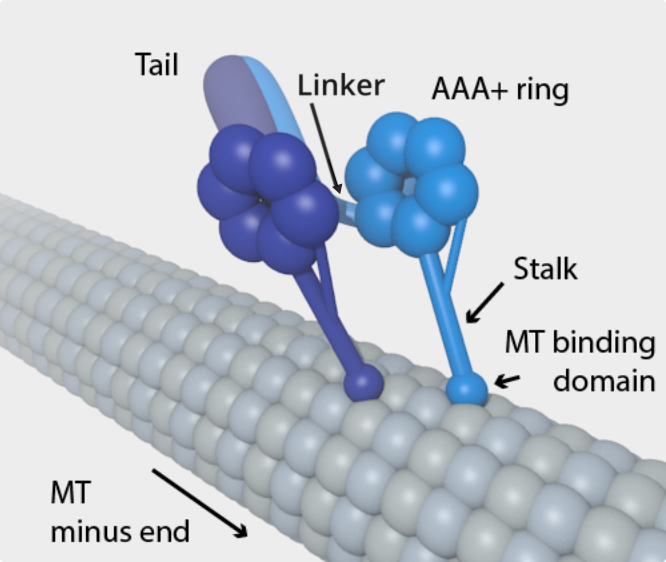
\includegraphics[width=0.6\columnwidth]{Figures/dynein_on_MT.png}
	\caption[Dynein on Microtubule]{\textbf{Dynein on Microtubule} Artist’s illustration of a dimer of cytoplasmic dynein heavy chains bounded to microtubule. This rendition similarly illustrates dynein’s structure as a domain-rod system, where the unlabeled linker domain connects the two AAA+ domains to the tail. \cite{TheTrappistArt}}
	\label{fig:final_disp}
\end{figure}


\section{Functions}
\textit{Purpose in the cell. What does dynein do that helps the cell operate? It walks on microtubule towards minus end. It uses chemical energy from ATP hydrolysis to convert into mechanical energy to walk and transport cargo with information along the cell. }

\begin{figure}[H]
	\centering
	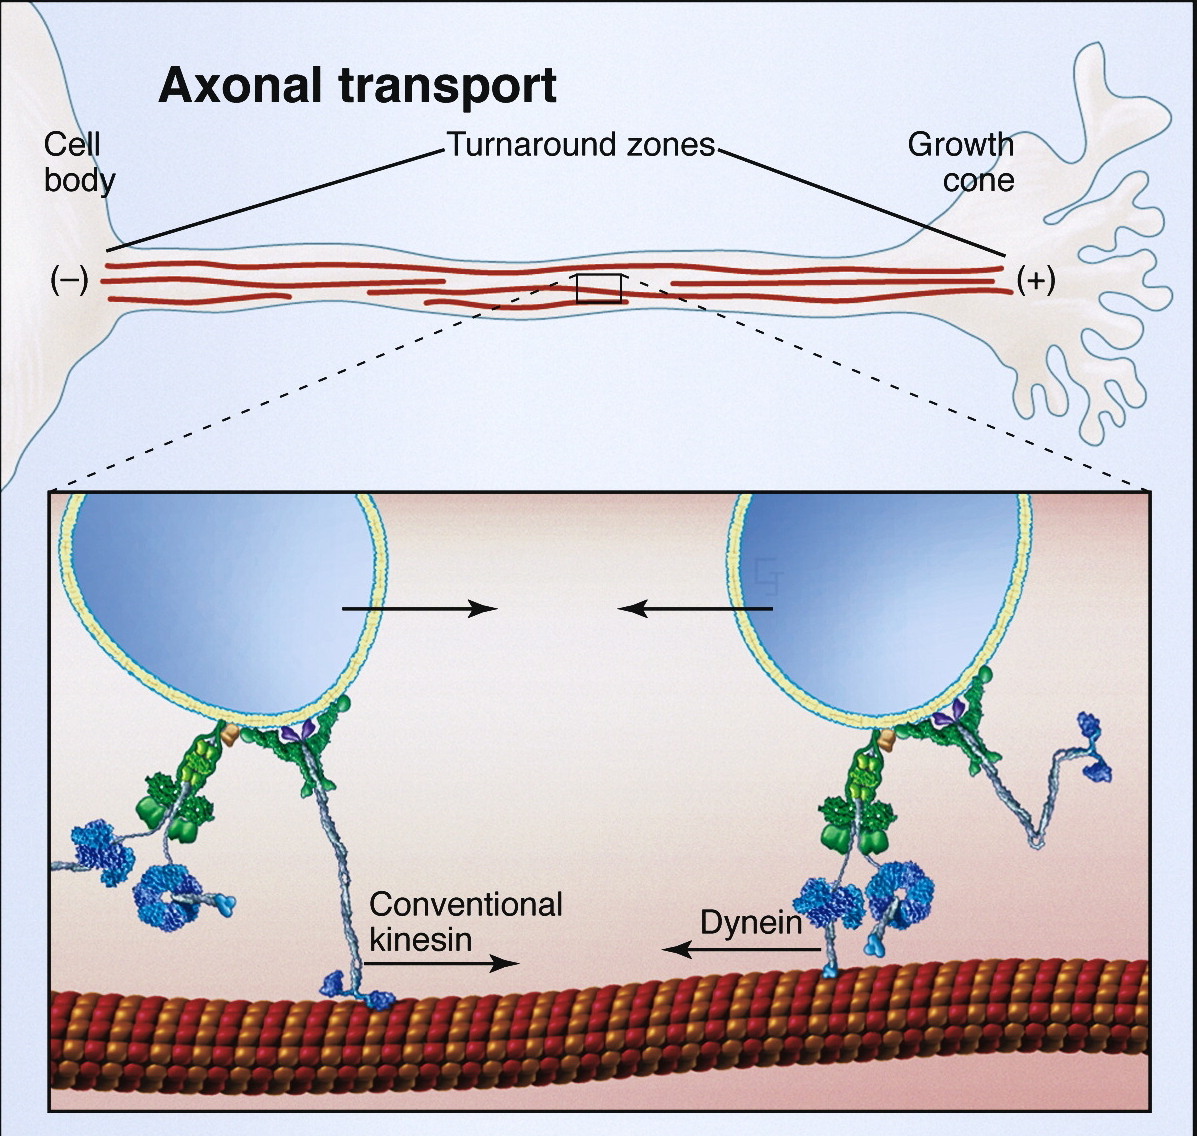
\includegraphics[width=0.6\columnwidth]{Figures/retrograde_transport.jpg}
	\caption[Retrograde Transport]{\textbf{Retrograde Transport} \cite{Vale2003molecular}}
	\label{fig:transport}
\end{figure}


\section{Architecture}
\textit{In-detail background knowledge on structure of dynein. Talk about each domain and their roles. Binding domain, six AAA+ domains, tail, and cargo. Stalk and linker that attaches things together. How the structure is so much larger than that of kinesin. dynein has flexibility because of its linker and in order to compensate for its huge domains. }

\begin{figure}[H]
	\centering
	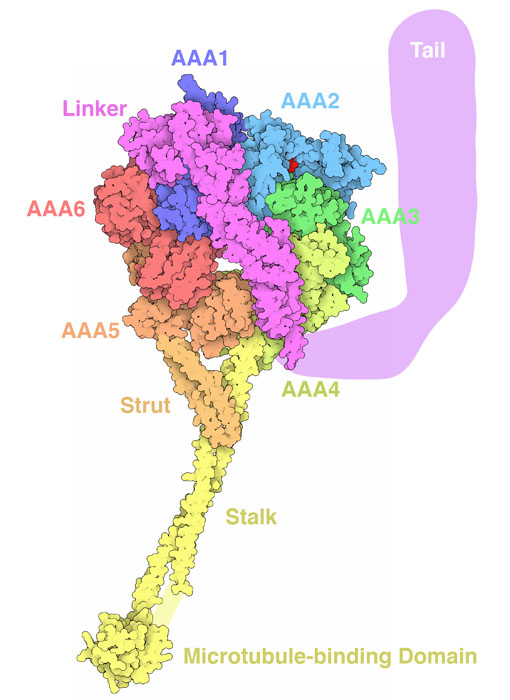
\includegraphics[width=0.6\columnwidth]{Figures/dynein_polypeptide.jpg}
	\caption[Polypeptide Structure]{\textbf{Polypeptide Structure} \cite{GoodsellArt}}
	\label{fig:polypeptide}
\end{figure}


\section{Stepping}
\textit{Biology and chemistry of stepping. What is actually causing it to step? ATP hydrolysis. Maybe short introduction on stepping and go more in detail in Power Stroke model. Say there are multiple theories and models of how dynein steps. Powerstroke, Winch, etc. Power stroke is most accepted. It can step on microtubule that is made up of tubulin dimers, $\alpha$ and $\beta$ tubulins. They are normally 8nm apart and so experimentalists believe dynein average step is always factor of 8nm. }


\begin{figure}[H]
	\centering
	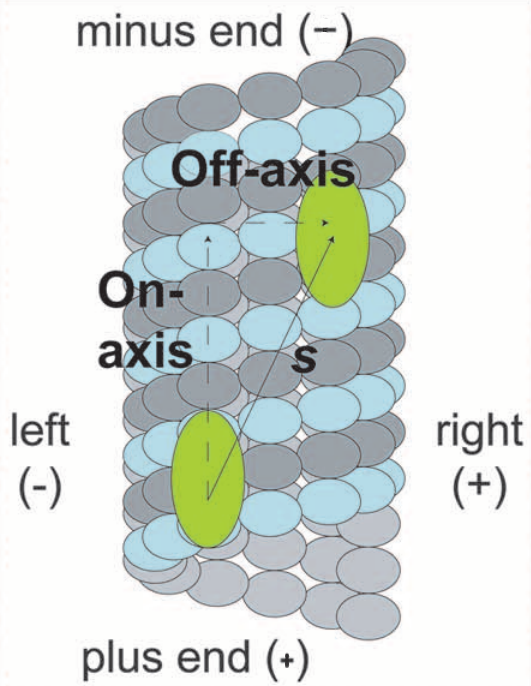
\includegraphics[width=0.3\columnwidth]{Figures/Onaxis.png}
	\caption[Stepping Axis]{\textbf{Stepping axis}  \cite{Dewitt2012} }
	\label{fig:YildizCorrelation}
\end{figure}


\subsection{Powerstroke Model}
\textit{Theorized model of stepping. Mechanochemical Cycle. Talk about ATP hydrolysis. Different conformational changes within a step. Look at linker and how it changes angles. Physically, it looks like it unbinds, stretches leg, then kicks forward, then diffuse back to MT.} 

\begin{figure}[H]
	\centering
	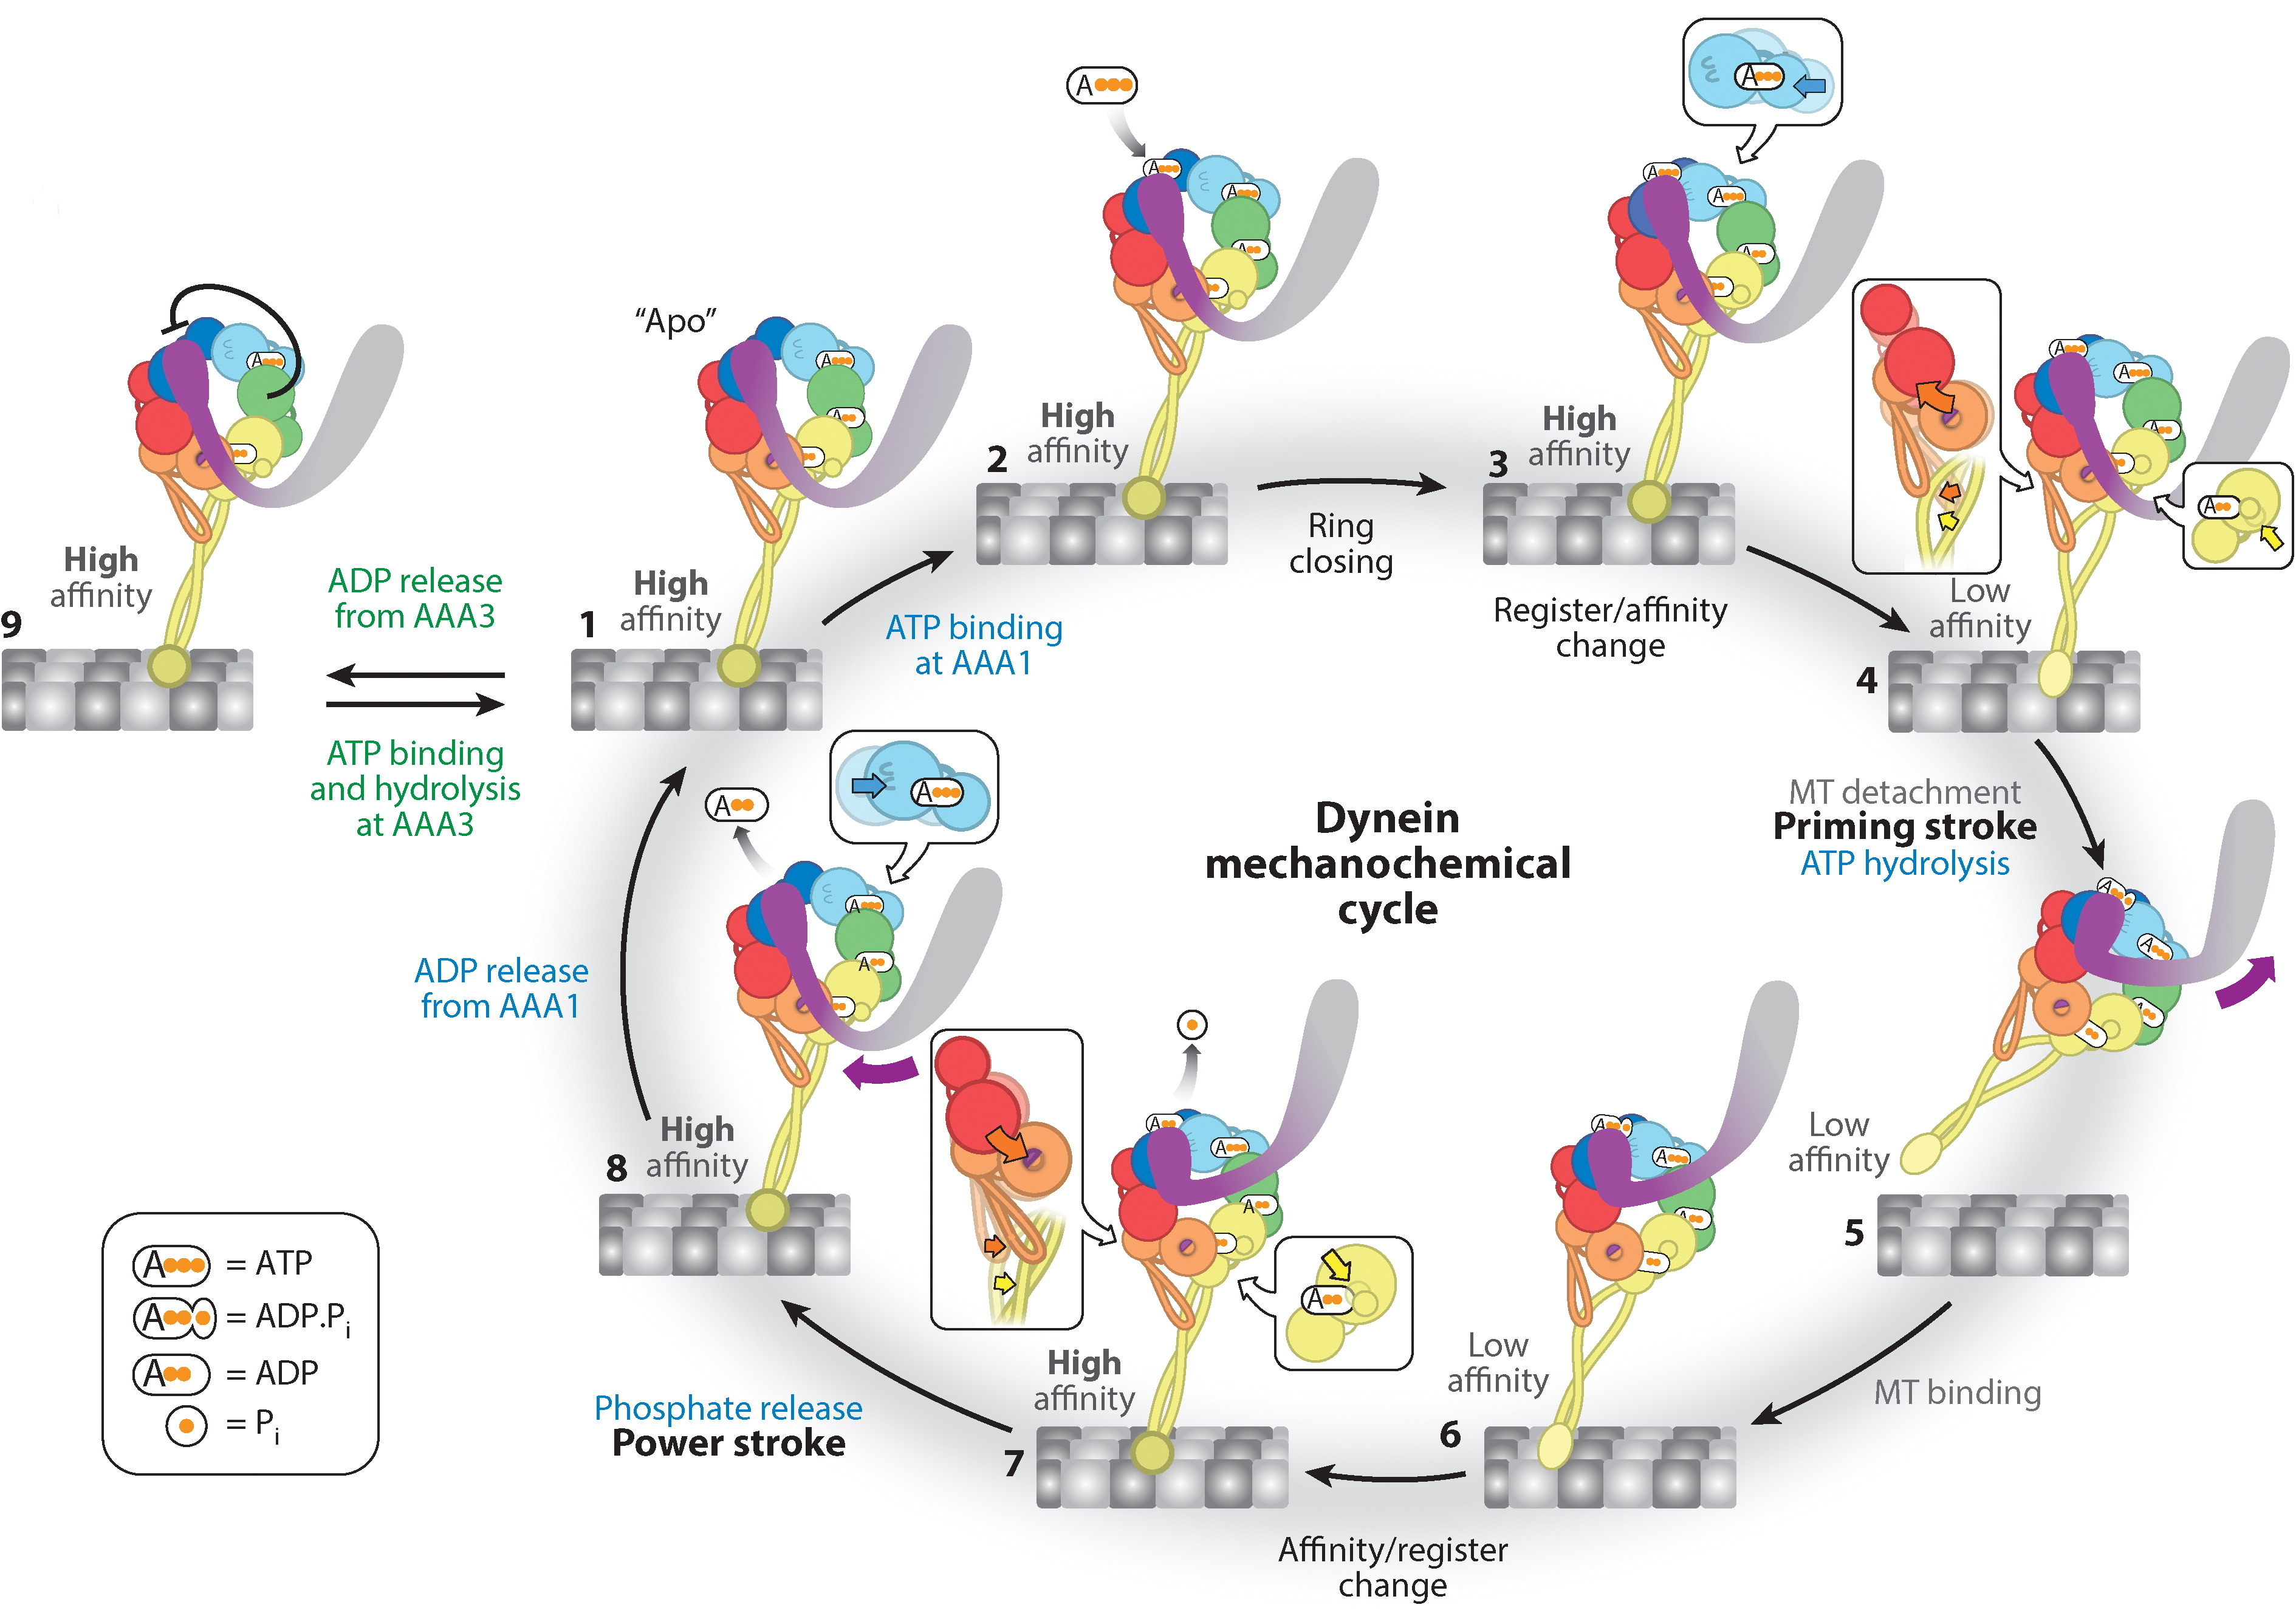
\includegraphics[width=1\columnwidth]{Figures/mechanochemical_cycle.jpeg}
	\caption[Mechanochemical Cycle]{\textbf{Mechanochemical Cycle}  \cite{Cianfrocco2015mechanism}}
	\label{fig:MechanochemicalCycle}
\end{figure}

\begin{figure}[H]
	\centering
	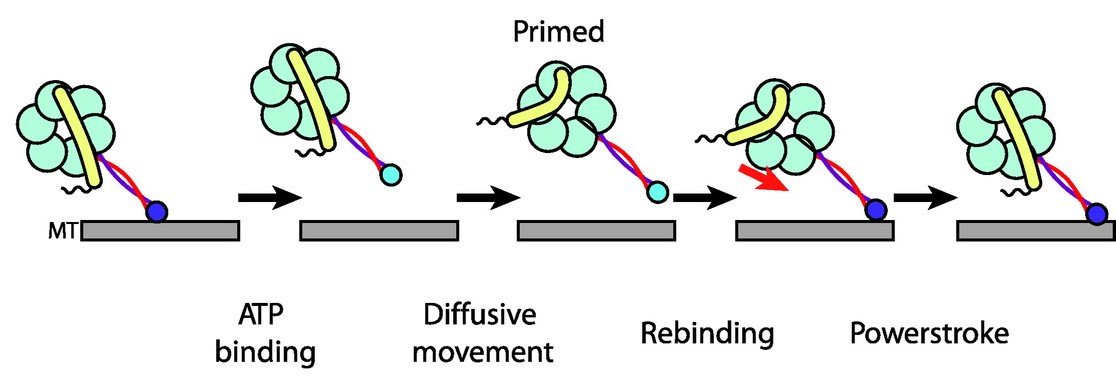
\includegraphics[width=1\columnwidth]{Figures/powerstroke.jpeg}
	\caption[Powerstroke]{\textbf{Powerstroke}  \cite{Carter2010communication} }
	\label{fig:Powerstroke}
\end{figure}


\section{Experimental Research on Dynein}
\textit{Most likely just short sections on experiments done on dynein.}
\subsection{Measuring}
\textit{How are experimentalists measuring dyneins stepping? Quantum dots on motor domains or quantum rod on tail, etc. }

\subsection{Interhead Coordination}
\textit{Purpose of my research. Trying to make model and fit to Yildiz analysis of dynein having interstep correlation. Dependency between step length and initial inter head separation.}

\begin{figure}[H]
	\centering
	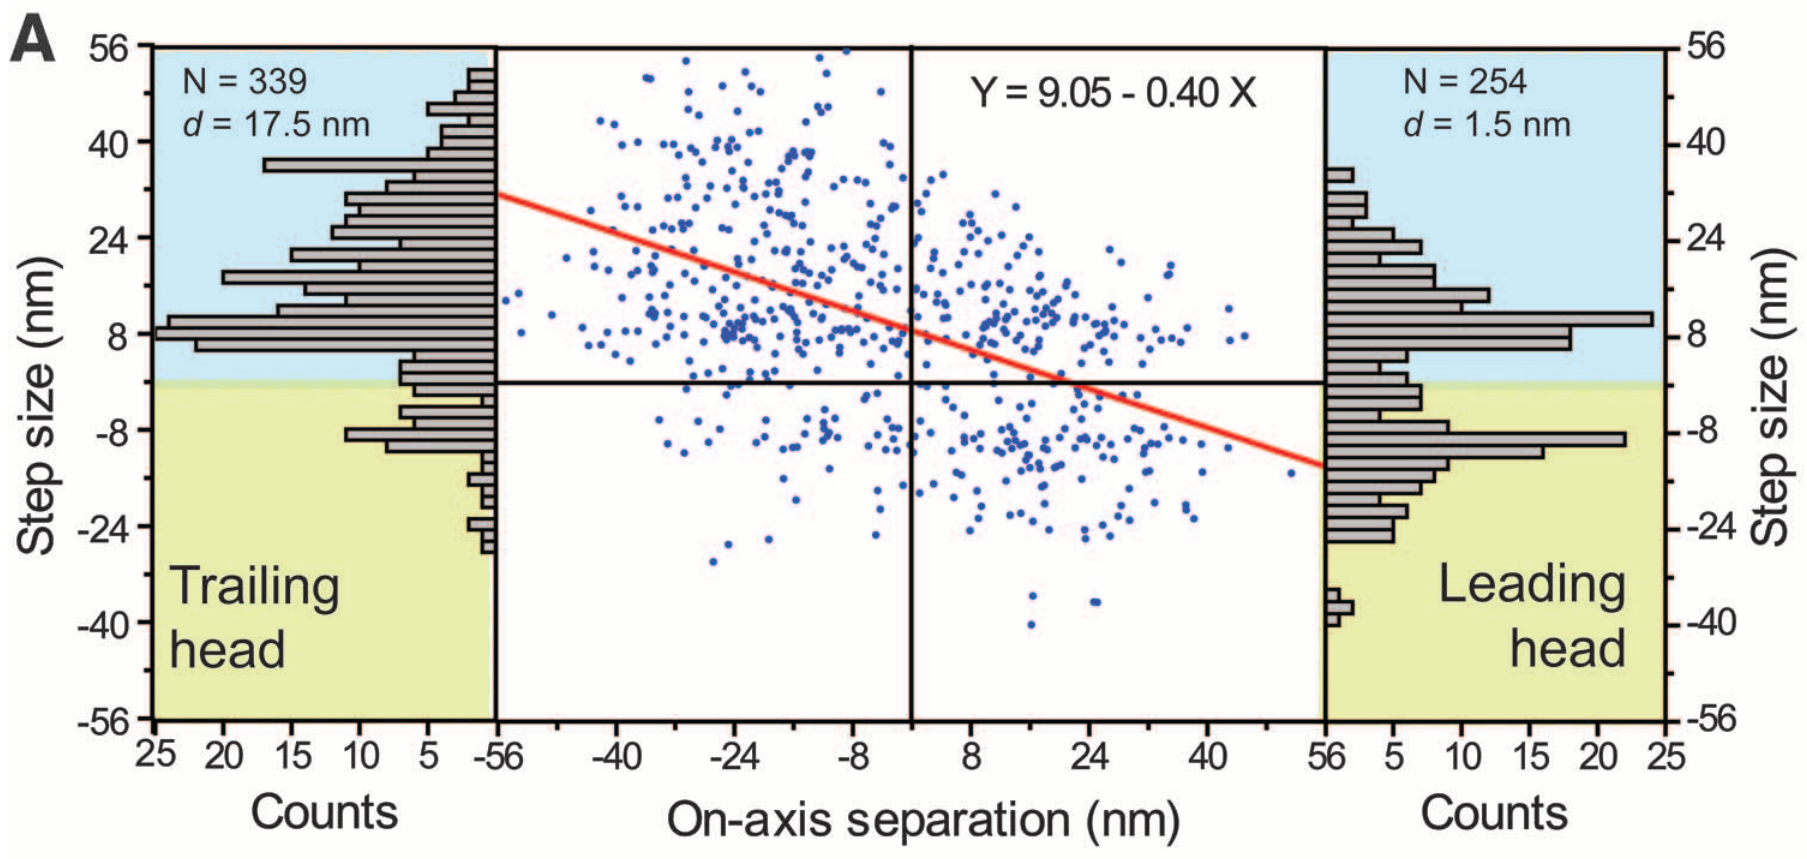
\includegraphics[width=1\columnwidth]{Figures/Yildiz_stepping.png}
	\caption[Stepping Correlation]{\textbf{Stepping Correlation}  \cite{Dewitt2012} }
	\label{fig:YildizCorrelation}
\end{figure}
